\section{Part II: Evaluation}

\begin{frame}{Benchmark NIDS datasets — A Closer Look}

	\small
	\begin{columns}[T,onlytextwidth]
		\column{0.55\linewidth}
		\begin{itemize}
			\item A single source dataset partitioned into \(\mathcal{D}_{\text{train}}\)
			      and \(\mathcal{D}_{\text{test}}\).
			\item Reported evaluation accuracies >\ \textbf{90\%} in published works on
			      public benchmarks (IDS2017, UNSW-NB15…) \(\rightarrow\) solved problem or
			      benchmark-induced illusions?
			\item A near-complete overlap of DoS-Hulk flows in IDS2017's
			      \(\mathcal{D}_{\text{train}}\) and \(\mathcal{D}_{\text{test}}\)\footnotemark.

		\end{itemize}

		\vspace{2em}

		\setbeamercolor{focusbox}{use={structure, normal text},
			fg=structure.fg,
			bg=structure.fg!12!normal text.bg}
		\begin{beamercolorbox}[wd=\linewidth, sep=1ex, rounded=true]{focusbox}
			\small Overlap between \(\mathcal{D}_{\text{test}}\) and
			\(\mathcal{D}_{\text{train}}\) does not prevent overfitting
			\(\rightarrow\) it can hide it.
		\end{beamercolorbox}

		\column{0.4\linewidth}
		\begin{figure}
			\centering
			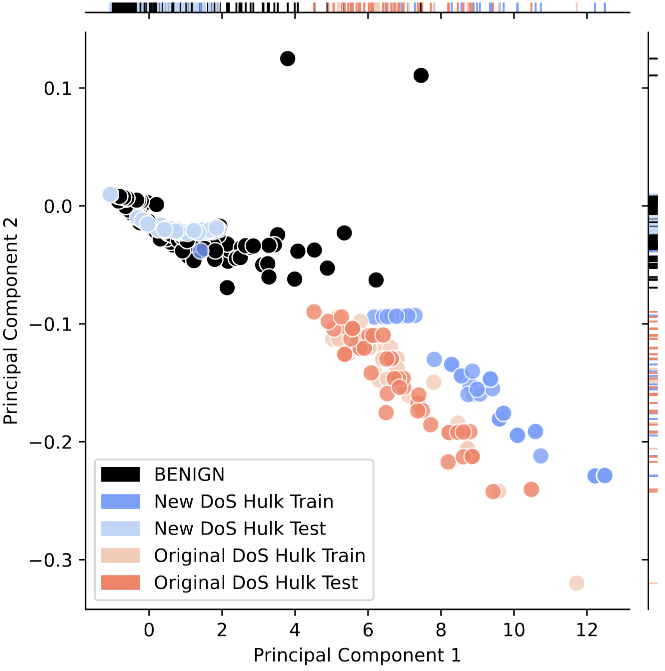
\includegraphics[width=\linewidth]
			{figures/TATA/bad_smells}
			\label{fig:bad_smells}
		\end{figure}
	\end{columns}

	\vspace{1em}
	\footnotetext{\tiny Flood et al., Bad Design Smells in Benchmark NIDS
		Datasets, IEEE EuroS\&P 2024.}

\end{frame}


\begin{frame}{Focusing on \(\mathcal{D}_{\text{test}}\) and its relation to \(\mathcal{D}_{\text{train}}\)}
	\small
	\begin{columns}[T,onlytextwidth]
		\column{0.42\linewidth}
		\begin{itemize}
			\item A robust evaluation should expose challenging cases, including
			      corner cases.
			\item Pre-deployment evaluation mainly relies on the test set
			      \(\mathcal{D}_{\text{test}}\).
			\item The key question is whether \(\mathcal{D}_{\text{test}}\)
			      really stresses the ML-based NIDS.
			\item The detector is constructed from
			      \(\mathcal{D}_{\text{train}}\) \( \rightarrow \)
			      \(\mathcal{D}_{\text{test}}\) must be assessed relative to
			      \(\mathcal{D}_{\text{train}}\).
		\end{itemize}

		\column{0.56\linewidth}
		\centering
		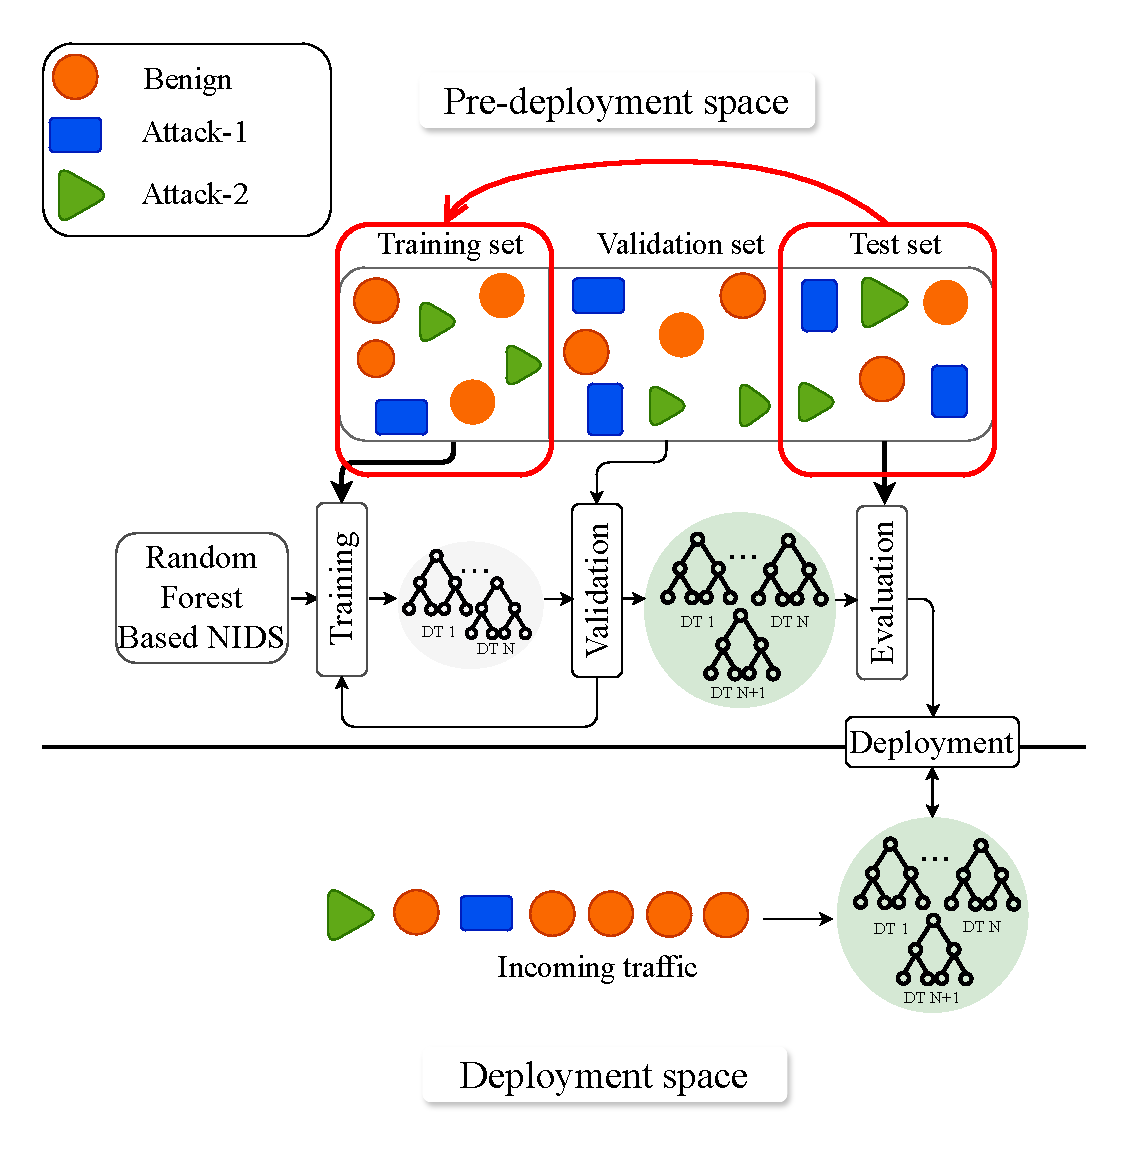
\includegraphics[width=\linewidth,height=0.8\textheight,keepaspectratio]{figures/TATA/ML_NIDS_last.pdf}
	\end{columns}

	\vspace{0.2em}
	\centering
	\textbf{$\Rightarrow$ This part focuses on \(\mathcal{D}_{\text{test}}\) and its relation to \(\mathcal{D}_{\text{train}}\).}

\end{frame}



% ---------- add in the preamble -----------------
% custom colours for the two RQs
\definecolor{rqblue}{RGB}{  0, 86,123}
\definecolor{rqgreen}{RGB}{  0,123, 86}

% use them for beamer blocks
\setbeamercolor{block title}{fg=white,bg=rqblue}
\setbeamercolor{block title alerted}{fg=white,bg=rqgreen}


% ------------ RQ slide -------------
\begin{frame}{Research Questions}
	\vspace{0.5em}

	\begin{block}<2->{\Large RQ1 — Test-set Assessment}

		\large How can we create a numerical score or a set of metrics to objectively
		measure the difficulty of a \(\mathcal{D}_\text{test}\) for a NIDS?

	\end{block}


	\vspace{3em}

	\begin{block}<1->{\Large RQ2 — Targeted Augmentation}

		\large Given a \textbf{too-easy} initial $\mathcal{D}_\text{test}$, can we apply
		systematic augmentation to generate new, \textbf{realistic}, and
		\textbf{challenging} traffic that is specifically designed to expose the hidden
		weaknesses of the NIDS?

	\end{block}


\end{frame}

\newcommand{\limMA}{\begingroup\large\faUnlock\endgroup}
%\newcommand{\limNN}{\begingroup\large\faMicrochip\endgroup}
\newcommand{\limTA}{\begingroup\large\faRuler\endgroup}
\newcommand{\limRT}{\begingroup\large\faRedo\endgroup}
\newcommand{\limSY}{\begingroup\large\faFlask\endgroup}
\newcommand{\limPR}{\begingroup\large\faBullseye\endgroup}
\newcommand{\limMU}{\begingroup\large\faHandPointer\endgroup}
\newcommand{\limMC}{\begingroup\large\faTools\endgroup}
\newcommand{\gOne}[1]{\colorbox{blue!15}{#1}}
\newcommand{\gTwo}[1]{\colorbox{green!20}{#1}}
\newcommand{\gThree}[1]{\colorbox{orange!50}{#1}}
% usage: \lateGOne{\limMA}
\newcommand{\lateGOne}[1]{\alt<12->{\gOne{#1}}{#1}}
\newcommand{\lateGTwo}[1]{\alt<12->{\gTwo{#1}}{#1}}
\newcommand{\lateGThree}[1]{\alt<12->{\gThree{#1}}{#1}}
\newcommand{\showat}[2]{\alt<#1->{#2}{\phantom{#2}}}
\newcommand{\finalonly}[1]{\alt<4->{#1}{\phantom{#1}}}
\newcommand{\ncovlim}{%
	\parbox[t]{\linewidth}{%
		Model access (\lateGOne{\limMA}) + NN-only (\lateGOne{\iconNN}) + \\
		Ignores train--test alignment (\lateGTwo{\limTA})}}

\newcommand{\ncovlimbf}{%
	\parbox[t]{\linewidth}{%
		\textbf
		{Model access (\lateGOne{\limMA}) + NN-only (\lateGOne{\iconNN}) + \\
			Ignores train--test alignment (\lateGTwo{\limTA})}}}
\newcommand{\ncovlimfinal}{%
	\parbox[t]{\linewidth}{%
		Model access (\gOne{\limMA}) + NN-only (\gOne{\iconNN}) + \\
		Ignores train--test alignment (\gTwo{\limTA})}}

\newcommand{\tataGapClosureVisual}{%
	\begin{tikzpicture}[baseline=(current bounding box.center)]
		\node[draw=black!15,fill=black!3,rounded corners=6pt,inner sep=5pt,align=center] (prior) at (0,0) {%
			\begin{minipage}{3.35cm}
				\centering
				{\scriptsize \textbf{Prior gaps}}\\[0.2em]
				{\scriptsize \gOne{\textbf{G1}}~\limMA~\iconNN~\limMC}\\[-0.05em]
				{\scriptsize \gTwo{\textbf{G2}}~\limTA~\limPR}\\[-0.05em]
				{\scriptsize \gThree{\textbf{G3}}~\limRT~\limSY~\limMU}
			\end{minipage}};
		\draw[red!75!black,line width=1.25pt] ([xshift=3pt,yshift=1pt]prior.south west) -- ([xshift=-3pt,yshift=-1pt]prior.north east);
		\node[anchor=west,draw=structure.fg,fill=structure.fg!10,rounded corners=6pt,inner sep=5pt,align=center] (tata) at (2.35,0) {%
			\begin{minipage}{2.35cm}
				\centering
				{\scriptsize \textbf{TATA closes}}\\[0.2em]
				{\scriptsize \gOne{\textbf{G1}}\hspace{0.45em}\gTwo{\textbf{G2}}\hspace{0.45em}\gThree{\textbf{G3}}}
			\end{minipage}};
		\draw[->,line width=0.9pt,draw=structure.fg] (prior.east) -- (tata.west);
	\end{tikzpicture}}
%% ------------------------------------------------------------
%\begin{frame}[c]{Related Work}
%    \centering
%
%    % helper icons
%    \newcommand{\cmark}{\textcolor{green!60!black}{\faCheck}}
%    \newcommand{\xmark}{\textcolor{red}{\faTimes}}
%
%    % table style
%    \scriptsize
%    \setlength{\tabcolsep}{10pt}
%    \renewcommand{\arraystretch}{2}
%
%    % ----------------------------------------------------------------
%    \begin{tabularx}{\linewidth}
%    {@{}>{\raggedright\arraybackslash}p{3.8cm} c c X@{}}
%        \toprule
%        \textbf{Method category} & \textbf{RQ1} & \textbf{RQ2} &
%        \textbf{Key limitations} \\
%        \midrule
%
%
%        % ---------------------------------------------
%        \only<1>{\phantom{Neuron coverage}}%
%        \only<2->{Neuron coverage} &
%
%        \only<1>{\phantom{\cmark}}%
%        \only<2->{\cmark} &
%
%        \only<1>{\phantom{\xmark}}%
%        \only<2->{\xmark} &
%
%        \only<1>{\phantom{\ncovlim}}%   % reserves height on overlay 1
%        \only<2>{\ncovlim}%              % normal on overlay 2
%        \only<3>{\ncovlimbf}%            % bold on overlay 3
%        \only<4->{\ncovlim}%             % normal again from overlay 4
%        \\[0.3em]
%
%
%        % Row 2 — Surprise coverage ------------------------------------
%        \only<1-3>{\phantom{Surprise coverage}}%
%        \only<4->{Surprise coverage} &
%        \only<1-3>{\phantom{\cmark}}%
%        \only<4->{\cmark} &
%        \only<1-3>{\phantom{\xmark}}%
%        \only<4->{\xmark} &
%        \only<1-3>{
%            \phantom
%            {\limMA \; + \; \iconNN \; + \; Proximity-only
%            focus (\lateGTwo{\limPR})}}%
%        \only<4>
%        {\limMA \; + \; \iconNN \; + \; Proximity-only
%        focus (\lateGTwo{\limPR})}
%        \only<5>{
%            \textbf
%            {\limMA \; + \; \iconNN \; + \; Proximity-only
%            focus (\lateGTwo{\limPR})}}
%        \only<6->
%        {\limMA \; + \; \iconNN \; + \; Proximity-only
%        focus (\lateGTwo{\limPR})}%
%        \\[0.3em]
%
%        % Row 3 — Mutation testing -------------------------------------
%        \only<1-5>{\phantom{Mutation testing}}%
%        \only<6->{Mutation testing} &
%        \only<1-5>{\phantom{\cmark}}%
%        \only<6->{\cmark} &
%        \only<1-5>{\phantom{\xmark}}%
%        \only<6->{\xmark} &
%        \only<1-5>
%        {
%            \phantom
%            {\limMA \; + \; \limTA \; + \; Model-change
%            sensitive (\lateGOne{\limMC})}}%
%        \only<6>
%        {\limMA \; + \; \limTA \; + \; Model-change
%        sensitive (\lateGOne{\limMC})}%
%        \only<7>{\textbf
%        {\limMA \; + \; \limTA \; + \; Model-change
%        sensitive (\lateGOne{\limMC})}}%
%        \only<8->
%        {\limMA \; + \; \limTA \; + \; Model-change
%        sensitive (\lateGOne{\limMC})}%
%        \\[0.3em]
%
%        % Row 4 — DeepMETIS --------------------------------------------
%        \only<1-7>{\phantom{Mutation testing (DeepMetis)}}%
%        \only<8->{Mutation testing (Deepmetis)} &
%        \only<1-7>{\phantom{\cmark}}%
%        \only<8->{\cmark} &
%        \only<1-7>{\phantom{\cmark}}%
%        \only<8->{\cmark} &
%        \only<1-7>{
%            \phantom
%            {Retrain per dataset (\lateGThree{\limRT}) \;+\;Synthetic
%            data (\lateGThree{\limSY})}}%
%        \only<8>
%        {Retrain per dataset (\lateGThree{\limRT}) \;+\;Synthetic
%        data (\lateGThree{\limSY})}%
%        \only<9>{
%            \textbf
%            {Retrain per dataset (\lateGThree{\limRT}) \;+\;Synthetic
%            data (\lateGThree{\limSY})}}%
%        \only<10->
%        {Retrain per dataset (\lateGThree{\limRT}) \;+\;Synthetic
%        data (\lateGThree{\limSY})}%
%        \\[0.3em]
%
%        % Row 5 — Flood 2024 -------------------------------------------
%        \only<1-9>{\phantom{Manual}}%
%        \only<10->{Manual (\cite{flood2014baddesign})} &
%        \only<1-9>{\phantom{\xmark}}%
%        \only<10->{\xmark} &
%        \only<1-9>{\phantom{\cmark}}%
%        \only<10->{\cmark} &
%        \only<1-9>{
%            \phantom{Unguided augmentation (\lateGThree{\limMU})}}%
%        \only<10>
%        {Unguided augmentation (\lateGThree{\limMU})}%
%        \only<11>{
%            \textbf{Unguided augmentation (\lateGThree{\limMU})}}%
%        \only<12->
%        {Unguided augmentation (\lateGThree{\limMU})}%
%        \\
%
%        \bottomrule
%    \end{tabularx}
%
%    % =========== Definition / Take-away card ========================
%    \vspace{1em}
%
%    % ---- normal definition card (overlays 1–11) --------------------
%    \only<1-11>{%
%        \begin{beamercolorbox}[rounded=true,shadow=true,wd=\linewidth,sep=1ex]
%        {defbox}
%            \scriptsize
%            \only<2-3>{\textbf{Neuron coverage: }
%            Fraction of neurons whose activation exceeds a preset threshold at least once
%            across the test set; higher $\rightarrow$ explore more of the model’s
%internal
%            logic.}
%            \only<4-5>
%            {\textbf{Surprise coverage: } Measures how broadly the test set differs from
%            what the model saw in training; higher $\rightarrow$ the set includes both
%            familiar and highly surprising inputs.}
%            \only<6-7>
%            {
%            \textbf{Mutation testing: } Mutates the model or its training setup (e.g.,
%            weights, architecture, or hyperparameters), then checks if the test set can
%            distinguish the mutant from the original model.}
%            \only<8-9>
%            {
%            \textbf{DeepMetis:} Combines mutation testing with synthetic data
%generation to
%            create new test data points that expose the mutated models’ weaknesses.}
%            \only<10-11>
%            {\textbf{Flood et al. 2024~\cite{flood2014baddesign}:} Manual generation
%of DoS-Hulk attacks with 60
%            randomised web-page-size (1–10 MB) ✚ bandwidth (1–50 Mbps) combinations, then
%            injected into IDS2017 to augment the test set}
%        \end{beamercolorbox}}
%
%    % ---- take-away card (overlay 12+) --------------------------------
%    \only<12->{%
%        \begin{beamercolorbox}[rounded=true,shadow=true,wd=\linewidth,sep=0
%        .8ex]
%        {takebox}
%            \gOne{\textbf{G1}}\;Model-related gaps\quad
%            \gTwo{\textbf{G2}}\;Shortcomings in assessing \(\mathcal{D}_{\text{test}}
%            $\rightarrow$ RQ1\quad
%            \gThree{\textbf{G3}}\;Weaknesses in \(\mathcal{D}_{\text{test}}\)'s
%            augmentation workflows $\rightarrow$ RQ2\\[0.4em]
%        \end{beamercolorbox}}
%\end{frame}


\begin{frame}[c]{Related Work}
	\centering
	\newcommand{\cmark}{\textcolor{green!60!black}{\faCheck}}
	\newcommand{\xmark}{\textcolor{red}{\faTimes}}

	\scriptsize
	\setlength{\tabcolsep}{10pt}
	\renewcommand{\arraystretch}{2}

	% -------- Progressive table (t0..t2) --------
	\only<1-3>{%
		\begin{tabular}{@{}>{\raggedright\arraybackslash}p{3.9cm} c c p{7.6cm}@{}}
			\toprule
			\textbf{Method category}                      & \textbf{RQ1} & \textbf{RQ2} & \textbf{Key limitations}
			\\
			\midrule
			% t0
			\showat{1}{Neuron coverage}                   &
			\finalonly{\cmark}                            &
			\finalonly{\xmark}                            &
			\finalonly{\ncovlim}                                                                                   \\[0.3em]

			% t1
			\showat{2}{Surprise coverage}                 &
			\finalonly{\cmark}                            &
			\finalonly{\xmark}                            &
			\finalonly{\limMA \; + \; \iconNN \; + \; Proximity-only focus (\lateGTwo{\limPR})}
			\\[0.3em]

			% t2 (two rows)
			\multirow{2}{=}{\showat{3}{Mutation testing}} &
			\multirow{2}{*}{\finalonly{\cmark}}
			                                              &
			\multirow{2}{*}{\finalonly{\cmark}}
			                                              &
			\finalonly{\limMA \; + \; \limTA \; + \; Model-change sensitive (\lateGOne{\limMC})}
			\\
			                                              &              &              & \finalonly
			{Retrain per dataset (\lateGThree{\limRT}) \;+\; Synthetic data (\lateGThree{\limSY}
			)}                                                                                                     \\[0.3em]

			% Manual row: reserved, shown only on final
			\showat{4}{Manual (Flood et al.)}             &
			\finalonly{\xmark}                            &
			\finalonly{\cmark}
			                                              &
			\finalonly{Unguided augmentation (\lateGThree{\limMU})}
			\\
			\bottomrule
		\end{tabular}
	}

	% -------- Final table (t3) — full, exactly like before --------
	\only<4->{%
		\begin{tabular}{@{}>{\raggedright\arraybackslash}p{3.9cm} c c p{7.6cm}@{}}
			\toprule
			\textbf{Method category}          & \textbf{RQ1}                            & \textbf{RQ2} &
			\textbf{Key limitations}
			\\
			\midrule
			Neuron coverage                   & \cmark                                  & \xmark       & \ncovlimfinal
			\\[0.3em]
			Surprise coverage                 & \cmark                                  & \xmark       & \limMA \; + \;
			\iconNN \; + \; Proximity-only focus (\gTwo{\limPR})                                                                                     \\[0.3em]
			\multirow{2}{=}{Mutation testing} & \multirow{2}{*}{\cmark}                 &
			\multirow{2}{*}{\cmark}
			                                  &
			\limMA \; + \; \limTA \; + \; Model-change sensitive (\gOne{\limMC})
			\\
			                                  &                                         &              & Retrain per dataset (\gThree{\limRT}) \;+\;
			Synthetic data (\gThree{\limSY})                                                                                                         \\[0.3em]
			Manual (Flood et al., 2024)       & \xmark                                  & \cmark
			                                  & Unguided augmentation (\gThree{\limMU})
			\\
			\bottomrule
		\end{tabular}

		\vspace{0.8em}
		\begin{beamercolorbox}[rounded=true,shadow=true,wd=\linewidth,sep=0.8ex]{takebox}
			\gOne{\textbf{G1}}\;Model-related gaps\quad
			\gTwo{\textbf{G2}}\;Shortcomings in assessing \(\mathcal{D}_{\text{test}}\)
			$\rightarrow$ RQ1\quad
			\gThree{\textbf{G3}}\;Weaknesses in \(\mathcal{D}_{\text{test}}\)
			augmentation workflows $\rightarrow$ RQ2
		\end{beamercolorbox}
	}

	% -------- Explainers (two lines; fixed height) --------
	\only<1>{\begin{beamercolorbox}[rounded=true,shadow=true,wd=\linewidth,sep=1ex]{defbox}
			\scriptsize
			\textbf{Neuron coverage:}
			Fraction of neurons whose activation exceeds a preset threshold at least once
			across the test set; higher $\rightarrow$
			explore more of the model’s internal
			logic.
		\end{beamercolorbox}}

	\only<2>{\begin{beamercolorbox}[rounded=true,shadow=true,wd=\linewidth,sep=1ex]{defbox}
			\scriptsize
			\textbf{Surprise coverage:}
			Measures how broadly the test set differs from
			what the model saw in training; higher $\rightarrow$ the test set includes
			highly surprising inputs.
		\end{beamercolorbox}}

	\only<3>{\begin{beamercolorbox}[rounded=true,shadow=true,wd=\linewidth,sep=1ex]{defbox}
			\scriptsize
			\textbf{Mutation testing:}
			Mutates the model and/or its training setup (e.g., weights, architecture, or
			hyperparameters), then checks if the test set can distinguish the mutant from
			the original model.
		\end{beamercolorbox}}

\end{frame}

%\begin{frame}{TATA — Three Connected Phases}

\begin{frame}
	{TATA (\textbf{T}est-set \textbf{A}ssessment \& \textbf{T}argeted \textbf{A}ugmentation)}

	%    \small

	% ---- Goal sentence ------------------------------------------------
	\textbf{Goal:} Close the gaps identified in related work and answer the
	research questions.



	\begin{enumerate}
		\item \textbf{Preliminary Phase} \hfill \gOne{\textbf{G1}}: \limMA\;
		      +\;\iconNN\;+\;\limMC\\

		      Approximate \(\mathcal{D_{\text{train}}}\)'s decision boundary while being model
		      agnostic

		\item[]
		\item
		      \textbf{Phase 1 – Assesses \(\mathcal{D}_{\text{test}}\)'s quality (\textbf{RQ1})}
		      \hfill
		      \gTwo{\textbf{G2}}: \limTA\;+\;\limPR\\

		      \textbf{Define} three metrics (\textbf{Proximity}, \textbf{Diversity}, and
		      \textbf{Scarcity}) to assess the \textbf{alignment} of
		      \(\mathcal{D}_\text{test}\) with respect to \(\mathcal{D}_{\text{train}}\)'s
		      distribution.

		\item[]
		\item \textbf{Phase 2 – \(\mathcal{D}_{\text{test}}\) Augmentation (\textbf{RQ2})}
		      \hfill
		      \gThree{\textbf{G3}}: \limRT\;+\;\limSY\;+\;\limMU\\
		      Reinforcement learning
		      (RL) guides a testbed to generate \textbf{realistic traffic}
		      that fills uncovered metric gaps, producing \textbf{a more challenging}
		      \( \mathcal{D}_{\text{test}} \).
	\end{enumerate}

\end{frame}

\newcommand{\stepbox}[2]{\alt<#1>{\boxed{#2}}{#2}}

\begin{frame}
	{Preliminary Phase: Approximating \(\mathcal{D}_\text{train}\)'s decision boundary}
	\small

	\begin{figure}
		\centering
		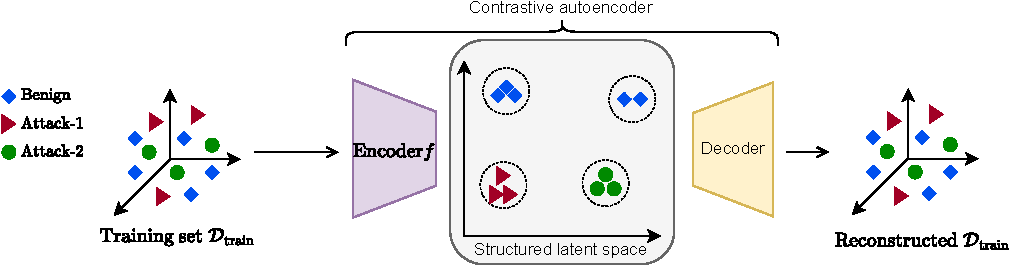
\includegraphics[width=\linewidth]{sections/TATA/methodology/figures/TATA_pre-crop}
		%    \caption*{
		%      \scriptsize{Encoder \(f\) and its associated decoder trained on
		%        \(\mathcal{D}_{\text{train}}\) to construct a structured latent
		%        space \(\mathcal{Z}_{\text{train}}=\{\,z \mid z=f(x;\theta),\ x\in
		%        \mathcal{D}_{\text{train}}\}\).}
		%    }
		\label{fig:tata_preliminary}
	\end{figure}

	\begin{itemize}
		%    \item Latent space under contrastive autoencoder: well-separated clusters
		%    \(C_{i,\,l_k} \in \mathcal{C}\); majority label \(l_k\) per cluster.
		%
		%    \item Dimensionality reduction; accelerated later phases; model-agnostic
		%    approximation of \(\mathcal{D}_{\text{train}}\) decision boundaries.

		\item Decision boundaries \(\approx\) cluster borders in the latent space; these
		      are captured in the encoder’s weights.

	\end{itemize}

\end{frame}

%\begin{frame}{Preliminary Phase: Approximating \(\mathcal{D}_\text{train}\)
%  's decision boundary}
%  \small
%  \begin{minipage}[t]{0.38\textwidth}
%    \begin{itemize}
%
%      \item Latent space under contrastive autoencoder: well-separated clusters
%      \(C_{i,\,l_k} \in \mathcal{C}\); majority label \(l_k\) per cluster.
%
%      \item Dimensionality reduction; accelerated later phases; model-agnostic
%      approximation of \(\mathcal{D}_{\text{train}}\) decision boundaries.
%
%    \end{itemize}
%  \end{minipage}
%  \hfill
%  \begin{minipage}[t]{0.6\textwidth}
%    \begin{figure}
%      \centering
%      
\includegraphics[width=1.1\linewidth]{tata/figures/TATA_pre-crop}
%      \caption*{
%        \scriptsize{Encoder \(f\) and its associated decoder trained on
%          \(\mathcal{D}_{\text{train}}\) to construct a structured latent
%          space \(\mathcal{Z}_{\text{train}}=\{\,z \mid z=f(x;\theta),\ x\in
%          \mathcal{D}_{\text{train}}\}\).}}
%      \label{fig:tata_preliminary}
%    \end{figure}
%  \end{minipage}
%\end{frame}

\begin{frame}{Phase 1: Test-set Assessment}
	\small
	\begin{minipage}[t]{0.48\textwidth}
		\begin{itemize}

			\item Encode $\mathcal{D}_{\text{train}}$ \& $\mathcal{D}_{\text{test}}$
			      $\rightarrow$ $\mathcal{Z}_{\text{test}}$ is located relative to
			      $\mathcal{Z}_{\text{train}}$ $\rightarrow$ we now work entirely in latent space
			      (\(\mathcal{Z}_{\text{train}},\mathcal{Z}_{\text{test}}\)).



			\item[]

			\item For each test embedding \(z\), we identify:
			      \begin{itemize}
				      \item \(P(z)\): the nearest \textbf{same-label cluster} (\emph{positive
					            cluster})
				      \item \(N(z)\): the nearest \textbf{different-label cluster} (\emph{negative
					            cluster})
			      \end{itemize}

			\item[]


			\item Define proximity, diversity, and scarcity per \(P(z)\)
			      ; then aggreate.

		\end{itemize}
	\end{minipage}
	\hfill
	\begin{minipage}[t]{0.48\textwidth}
		\begin{figure}
			\centering
			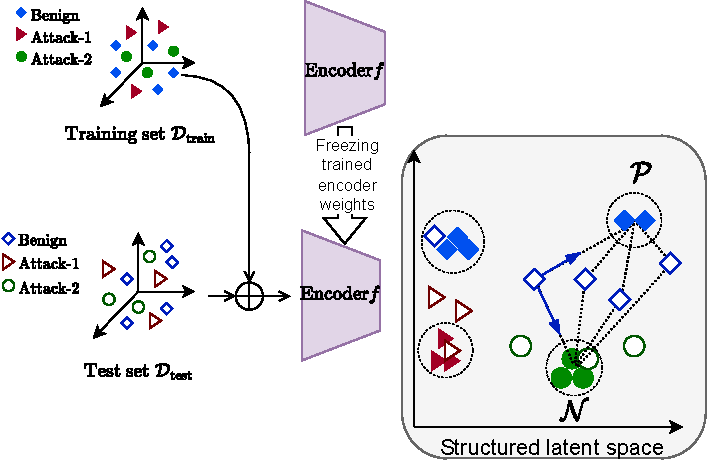
\includegraphics[width=\linewidth]
			{sections/TATA/methodology/figures/TATA_phase_1-crop}
			%      \caption*{\scriptsize{Assesing \(\mathcal{D}_{\text{test}}\) quality}}
			\label{fig:tata_phase_1}
		\end{figure}
	\end{minipage}
\end{frame}

\input{sections/TATA/methodology/metrics}


% --- Preamble (if not already added) ---
\newcommand{\strike}[1]{\textcolor{red!70!black}{\sout{#1}}}

% --- Frame ---
\begin{frame}{Which approaches can augment the test set?}
	\small

	\begin{enumerate}
		% 1) Synthetic generation (as before; crossed on next click)
		\item<1->
		      \alt<2->{\strike{GANs / diffusion models.}}
		      {GANs / diffusion models.}
		      \begin{itemize}
			      \item<2-> Synthetic generation may break protocol semantics $\Rightarrow$
			            unrealistic flows.
		      \end{itemize}

		      \vspace{0.6em}

		      % 2) Network simulators
		\item<3-> \alt<4->{\strike{Network simulators (e.g., NS-3, OMNeT++)}}
		      {Network simulators (e.g., NS-3, OMNeT++)}
		      \begin{itemize}
			      \item<4->
			            Models protocol interactions, offering more realism.
			      \item<4-> Remaining realism gap vs.\ real hardware and user behavior.
		      \end{itemize}

		      \vspace{0.6em}

		      % 3) Live testbed
		\item<5-> Using a \textbf{configurable live testbed}.
		      \begin{itemize}
			      \item<6-> Best preserves realism of generated traffic.
			      \item<6->
			            Emits legitimate traffic across multiple protocols (HTTP/HTTPS, SSH, SMTP, DNS,
			            \dots) and can generate attack traffic under controlled conditions.
		      \end{itemize}

		      \vspace{0.6em}

		      % This uncover block makes the colored box appear on the 9th click
		      \uncover<7->{
			      \setbeamercolor{focusbox}{use={structure, normal text},
			      fg=structure.fg,
			      bg=structure.fg!12!normal text.bg}
		      \begin{beamercolorbox}[wd=\linewidth, sep=1ex, rounded=true]{focusbox}
			      \small
			      Generate targeted configs so the testbed produces realistic flows targeting
			      under-covered \(\mathcal{Z}\) regions (low \(D,P,S\)).
		      \end{beamercolorbox}
		      }
	\end{enumerate}

\end{frame}

%\begin{frame}{Phase 2: Targeted Augmentation}
%  \scriptsize
%  \begin{minipage}[t]{0.52\textwidth}
%    \begin{itemize}
%
%      \item Start from Preliminary \& Phase 1 outputs
%      \item[]
%
%      \item \textbf{Train the agent (DRL):}
%
%      \begin{itemize}
%        \scriptsize
%        \item \textbf{Observation} \(o_t\): centroids \(\mathcal{C}\)
%        + basic stats of current \(\mathcal{Z}_{\text{test}}\)
%        (mean/min/max/var/std).
%        \item \textbf{Action} \(a_t\)
%        : select a testbed configuration (e.g., delay / loss / duplication).
%        \item \textbf{Reward} \(r_t\): \(D,P,S\).
%
%        \item \textbf{Training workflow}:
%        \[
%          \begin{aligned}
%            \stepbox{1}{o_t} &\;\to\; \stepbox{2}{a_t} \;\to\; \stepbox{3}{x_t}
%            \;\xrightarrow{\,f\,}\; \stepbox{4}{z_t} \;\to\;
%            \stepbox{5}{\text{update }\mathcal{Z}_{\text{test}}} \\
%            &\;\to\; \stepbox{6}{(r_t,\,o_{t+1})} \;\to\;
%            \stepbox{7}{\text{update }\pi}\;\stepbox{8}{\circlearrowright}
%            \;\Rightarrow\; \stepbox{9}{\pi^\ast}
%          \end{aligned}
%        \]
%
%      \end{itemize}
%
%      \item Apply \(\pi^\ast\) to augment any
%      \(\mathcal{D}_{\text{test}}\)
%    \end{itemize}
%  \end{minipage}
%  \hfill
%  \begin{minipage}[t]{0.47\textwidth}
%    \begin{figure}
%      \centering
%      
\includegraphics[width=1.1\linewidth]{tata/figures/TATA_phase_2_light-crop}
%%      \caption*{\scriptsize{Phase 2: targeted augmentation of
%%        \(\mathcal{D}_{\text{test}}\)
%%        using Preliminary + Phase 1 results.}}
%      \label{fig:tata_phase_2}
%    \end{figure}
%  \end{minipage}
%\end{frame}


\begin{frame}[t]{Phase 2: Targeted Augmentation}
	\scriptsize

	% --- top figure ---
	\begin{center}
		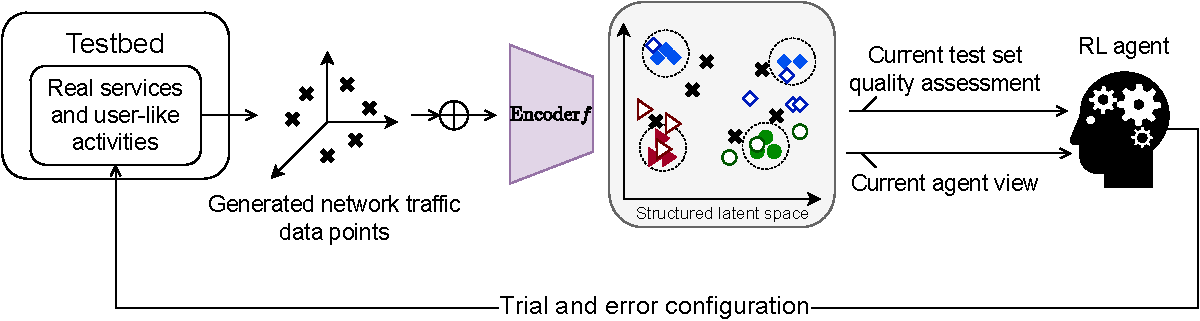
\includegraphics[width=0.95\linewidth]{sections/TATA/methodology/figures/TATA_phase_2_light-crop}
	\end{center}
	\vspace{0.4em}

	% --- text below ---
	\begin{itemize}
		\item Start from Preliminary \& Phase 1 outputs
		\item []
		\item \textbf{Training workflow}:
		      \[
			      \begin{aligned}
				      \stepbox{1}{\text{observe latent-space}} & \;\to\;
				      \stepbox{2}{\text{select a configuration}} \;\to\;
				      \stepbox{3}{\text{traffic generation}}
				      \;\xrightarrow{\;\text{embed}\;}\;
				      %        \stepbox{4}{\text{get latent embedding}} \;\to\; \\
				      \stepbox{4}{\text{update } \mathcal{Z}_{\text{test}}}                                                             \\
				                                               & \;\to\; \stepbox{5}{\text{compute proximity, diversity, and scarcity}}
				      \;\to\; \stepbox{6}{\text{update policy } \pi} \;\stepbox{7}{\circlearrowright}
				      \;\Rightarrow\; \stepbox{8}{\pi^\ast}
			      \end{aligned}
		      \]
		      %    \item []
		      %    \[
		      %      \begin{aligned}
		      %        \stepbox{1}{o_t} &\to \stepbox{2}{a_t} \to \stepbox{3}{x_t}
		      %        \xrightarrow{\,f\,} \stepbox{4}{z_t} \to
		      %        \stepbox{5}{\text{update }\mathcal{Z}_{\text{test}}}
		      %        &\to \stepbox{6}{(r_t,\,o_{t+1})} \to
		      %        \stepbox{7}{\text{update }\pi}\;\stepbox{8}{\circlearrowright}
		      %        \Rightarrow \stepbox{9}{\pi^\ast}
		      %      \end{aligned}
		      %    \]
		\item Apply \(\pi^\ast\) to augment any \(\mathcal{D}_{\text{test}}\)
	\end{itemize}
\end{frame}


%\begin{frame}{TATA}
%  \begin{figure}
%    \centering
%    \includegraphics[width=0.7\linewidth]
%    {tata/figures/TATA-crop}
%    \caption{Example Figure}\label{fig:tata_overview}
%  \end{figure}
%\end{frame}


% ------------------------------------------------------------
% Experimental Setup
% ------------------------------------------------------------
\begin{frame}{Experimental Setup}

	\scriptsize

	\textbf{Datasets (60 / 20 / 20 split)}

	\begin{itemize}
		\item [] \textit{(Using the revised and corrected versions)}
		\item \textbf{CIC-IDS 2017}: 0.93 M benign / 0.25 M attack flows
		\item \textbf{CSE-CIC-IDS 2018}: 59.8 M benign / 4.1 M attack flows
	\end{itemize}

	\textbf{NIDS Models}
	\begin{itemize}
		\item RF, SVM, 3-layer DNN (128-128-128 ReLU + Softmax)
	\end{itemize}

	%  \textbf{Latent-Space Encoder}
	%  \begin{itemize}
	%    \item 64 → 32 → 16 units, 3-D latent
	%  \end{itemize}

	\textbf{Agent Training}
	\begin{itemize}
		\item Augmentation targets Benign SSH flows only
		\item []
		\item Action space (client-side via \texttt{tc}):
		      \textbf{Loss} $\in [5,10]\%$ \ \textbar\
		      \textbf{Jitter} $\in [4,10]\,\mathrm{ms}$ \ \textbar\
		      \textbf{Delay} $\in [10,40]\,\mathrm{ms}$ \ \textbar\
		      \textbf{Duplication} $\in [0.1,5]\%$ \ \textbar\
		      \textbf{Corruption} $\in [0.1,10]\%$ \ \textbar\
		      \textbf{Reordering} $\in [0.1,50]\%$ \ \textbar\
		      \textbf{Correlation} $\in [50,100]\%$.
		      %    \item []
		      %    \item Offline RL dataset: \(\sim\)
		      %    500k transitions from IDS2018,
		      %    generated by uniformly sampling the action space while a scripted SSH
		      %    workload runs.

	\end{itemize}

\end{frame}


%\begin{frame}
%{Preliminary Phase — Latent Space Quality}
%  \small
%  \begin{itemize}
%    \item \textbf{Setup \& goal:} Contrastive vs.\
%    vanilla autoencoder on 10 random 60/20/20 splits of \textsc{IDS2017}/
%    \textsc{IDS2018}
%    ; aim is to evaluate the separability of the structured latent space.
%    \item \textbf{Silhouette:}
%    \textcolor{green!60!black}{+$\sim$0.22} (0.96–0.98 vs.\ 0.73–0.76)
%    \item \textbf{k-means accuracy:}
%    \textcolor{green!60!black}{+$\sim$39 pp} (99.90–99.99\% vs.\ 59.8–62.9\%)
%    \item \textbf{Takeaway:}
%    Contrastive forms tight, well-separated, label-pure clusters; vanilla shows
%    label mixing.
%  \end{itemize}
%\end{frame}


%================= PROXIMITY (in practice) =================
\begin{frame}{Proximity in Practice (IDS2017 only)}
	\small
	\begin{columns}[T,onlytextwidth]
		% Left: text
		\column{0.58\linewidth}
		\begin{itemize}
			\item Build 100 cumulative sub-tests by sorting \(z\) by distance to \(N(z)\).
			\item[]
			\item Beyond a proximity threshold, macro-F1 decreases as points close to decision
			      boundaries accumulate --- \textbf{strong negative correlation}.
			\item[]
			\item Trends align across RF/DNN/SVM \(\Rightarrow\) proximity is
			      \textbf{model-agnostic}.
			      %      \item Build 100 cumulative sub-tests by sorting \(z\) by distance to
			      %      \(N(z)\); higher proximity = closer to boundary.
			      %      \item Macro-F1 stays \(\approx 1.0\) up to proximity
			      %      \(\approx 0.11\text{--}0.14\), then declines to \(\approx 0.92\)
			      %      ; strong negative correlation.
			      %      \item Higher proximity \(\Rightarrow\)
			      %      lower macro-F1; trends align across RF/DNN/SVM.
		\end{itemize}
		% Right: figure
		\column{0.40\linewidth}
		\centering
		\begin{figure}
			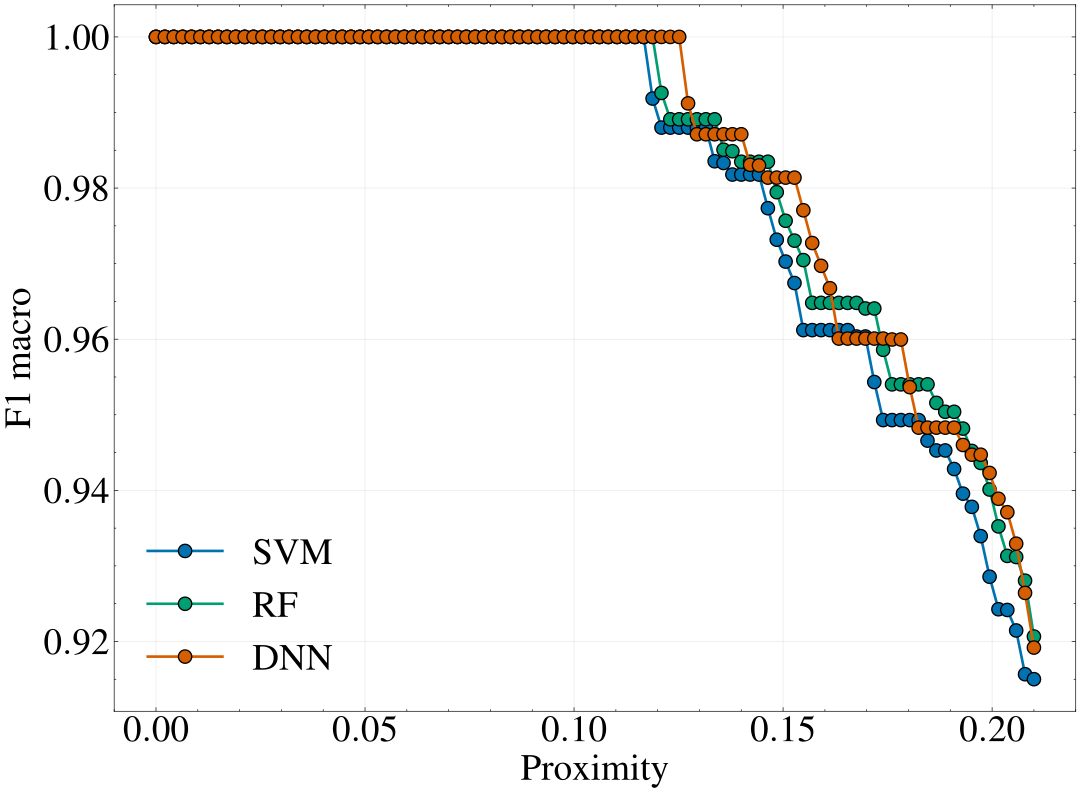
\includegraphics[width=0.95\linewidth]{sections/TATA/results/figures/proximity_in_practice-transparent.png}
			\caption{\scriptsize Macro-F1 vs. proximity across cumulative sub-tests (IDS2017).}
		\end{figure}
	\end{columns}
\end{frame}


%%================= DIVERSITY (in practice) =================
%\begin{frame}{Diversity in Practice (IDS2017 only)}
%  \small
%  \begin{columns}[T,onlytextwidth]
%    % Left: text
%    \column{0.58\linewidth}
%    \begin{itemize}
%      \item Sub-test sets: all label combinations of size \(k=1\ldots9\).
%      \item Diversity rises monotonically with \(k\); maximum \(\approx 0.1209\).
%      \item More traffic types \(\Rightarrow\) higher diversity \(\Rightarrow\)
%      more challenging evaluation.
%    \end{itemize}
%
%    % Right: figure
%    \column{0.40\linewidth}
%    \centering
%    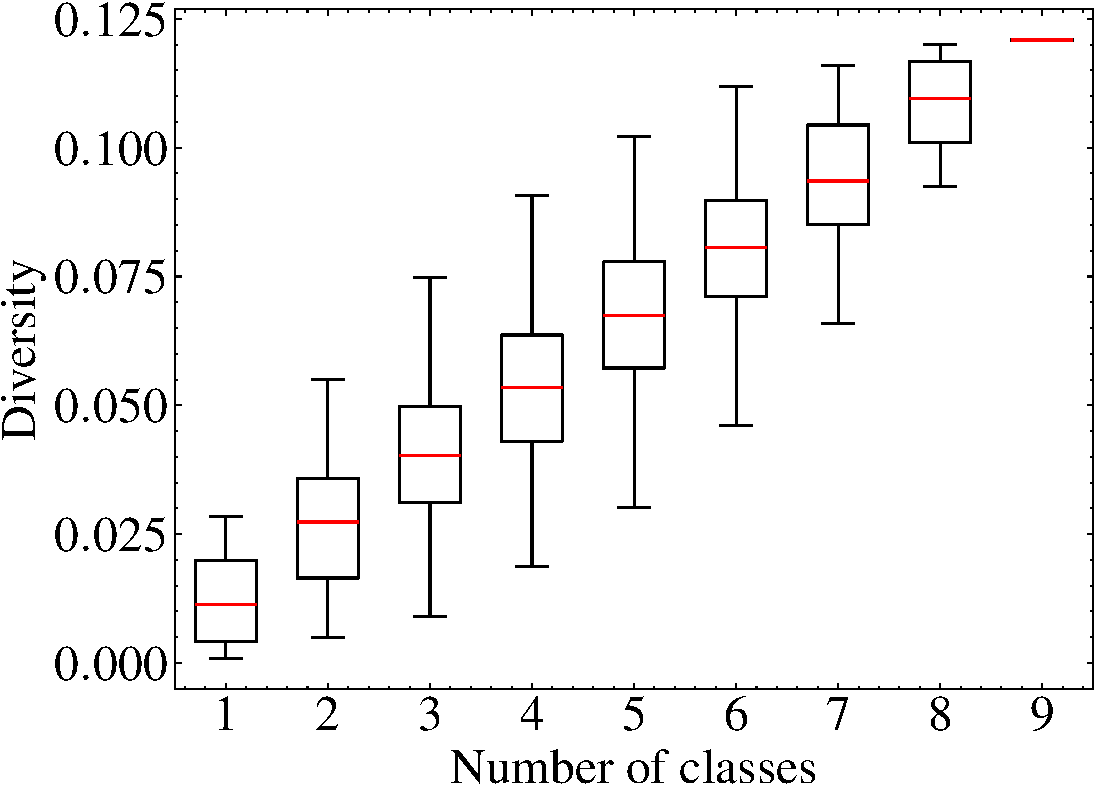
\includegraphics[width=\linewidth]{results/figures/diversity_boxplot-crop}
%  \end{columns}
%\end{frame}

%%================= SCARCITY (in practice) =================
%\begin{frame}{Scarcity in Practice (IDS2017 only)}
%  \small
%  \begin{columns}[T,onlytextwidth]
%    % Left: text
%    \column{0.58\linewidth}
%    \begin{itemize}
%      \item Increase scarcity by redistributing misclassified points across all negative
%      clusters in 10 steps.
%      \item
%      Macro-F1 drops sharply then monotonically; strong negative correlation; For
%      example, RF \(<0.78\) at scarcity \(\approx 0.53\).
%      \item More uniform spread across boundaries \(\Rightarrow\) higher scarcity
%      \(\Rightarrow\) lower macro-F1.
%    \end{itemize}
%
%    % Right: figure
%    \column{0.40\linewidth}
%    \centering
%    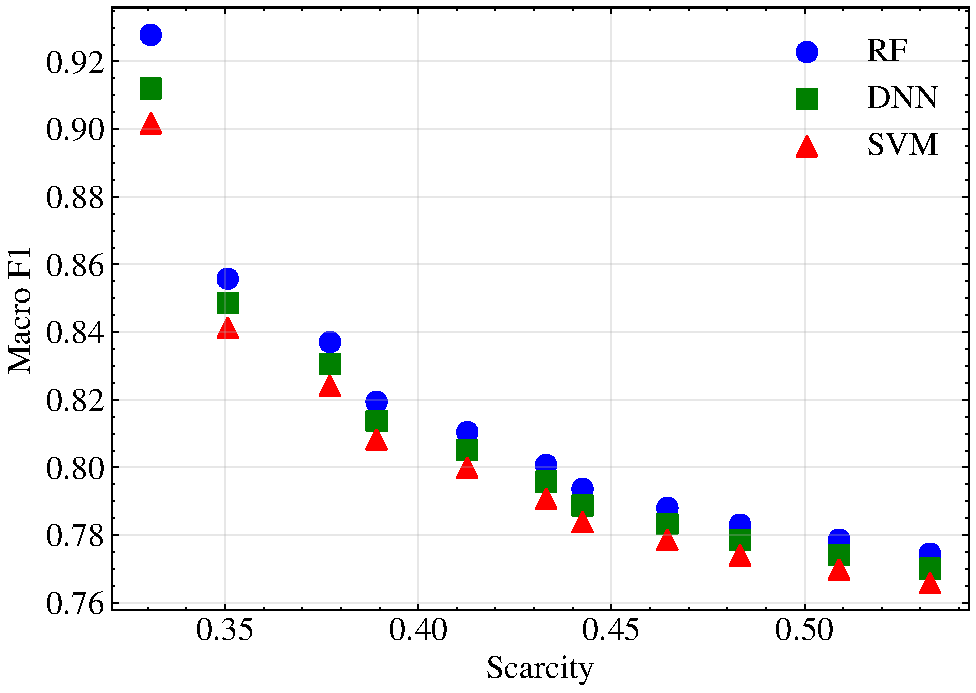
\includegraphics[width=0.95\linewidth]{results/figures/scarcity_in_practice}
%  \end{columns}
%\end{frame}

%\begin{frame}
%{Test set Augmentation Evaluation}
%
%  \scriptsize
%  \begin{columns}[T,onlytextwidth]
%    \column{0.55\linewidth}
%    \begin{itemize}
%      \item \textbf{Protocol:}
%      20 eval episodes on IDS2017; no reward/updates; add Benign SSH flows;
%      report mean$\pm$sd.
%      \item \textbf{Baselines:} Random, NetShare (GAN), RL\,+\,
%      Neuron Coverage (NC).
%      \item \textbf{Quality metrics:}
%      \begin{itemize}
%        \scriptsize
%        \item \textbf{TATA:} \(D\) \textcolor{green!60!black}{\(+\sim 437\%\)};
%        \(P\) \textcolor{green!60!black}{\(+\sim 190\%\)};
%        \(S\) \textcolor{green!60!black}{\(+\sim 136\%\)}
%        \item \textbf{NC:} \(D\) \textcolor{gray!60!black}{\(\approx 0\)};
%        \(P\) \textcolor{green!60!black}{\(+\sim 129\%\)};
%        \(S\) \textcolor{gray!60!black}{\(\approx 0\)}
%        \item \textbf{Random/NetShare:} \(D\)
%        \textcolor{red!70!black}{\(\downarrow\) to \(\approx 0\)};
%        \(P\) \textcolor{gray!60!black}{\(\approx 0\)};
%        \(S\) \textcolor{red!70!black}{\(\downarrow\)}
%      \end{itemize}
%
%      \item \textbf{NIDS impact:}
%      \begin{itemize}
%        \scriptsize
%        \item \textbf{TATA (RF example):} Precision
%        \textcolor{red!70!black}{–$\sim$46\%}; Recall
%        \textcolor{red!70!black}{–$\sim$13\%}
%        \item \textbf{NC (RF example):} Precision
%        \textcolor{red!70!black}{–$\sim$23\%}; Recall
%        \textcolor{red!70!black}{–$\sim$16\%}
%        \item \textbf{Note:} higher scarcity spreads errors across boundaries
%        $\Rightarrow$ FP $\uparrow$ $\Rightarrow$ precision $\downarrow$.
%      \end{itemize}
%
%    \end{itemize}
%
%    \column{0.42\linewidth}
%    \centering
%    \begin{figure}
%      \includegraphics[width=\linewidth]
%      {results/figures/bars_classifier_grayscale_std}
%      \caption*{\scriptsize
%      {Impact of TATA and Baselines on Test-Set Quality Metrics and Detection
%      Performance}}
%      \label{fig:test_set_aug_1}
%    \end{figure}
%  \end{columns}
%
%\end{frame}



\begin{frame}{Test-set Augmentation — Metrics}
	\small
	\begin{columns}[T,onlytextwidth]
		% ---------------- Left column ----------------
		\column{0.55\linewidth}
		\begin{itemize}
			\item<1-> \textbf{Protocol:}
			      20 eval episodes on IDS2017; no reward/updates; add Benign SSH flows;
			      report mean$\pm$sd.

			\item<1-> \textbf{Baselines:} Random, NetShare (GAN), RL\,+\,Neuron Coverage (NC).

			\item<2-> \textbf{Quality metrics:}
			      \begin{itemize}
				      \item<2-> \textbf{TATA:} \(D\) \textcolor{green!60!black}{\(+\sim 437\%\)}; \(P\)
				            \textcolor{green!60!black}{\(+\sim 190\%\)}; \(S\)
				            \textcolor{green!60!black}{\(+\sim 136\%\)}
				      \item<2-> \textbf{NC:} \(D\) \textcolor{gray!60!black}{\(\approx 0\)}; \(P\)
				            \textcolor{green!60!black}{\(+\sim 129\%\)}; \(S\)
				            \textcolor{gray!60!black}{\(\approx 0\)}
				      \item<2-> \textbf{Random/NetShare:} \(D\)
				            \textcolor{red!70!black}{\(\downarrow\) to \(\approx 0\)}; \(P\)
				            \textcolor{gray!60!black}{\(\approx 0\)}; \(S\)
				            \textcolor{red!70!black}{\(\downarrow\)}
			      \end{itemize}
		\end{itemize}

		% Step 3: prompt to transition
		\only<3->{%
			\begin{beamercolorbox}[rounded=true,shadow=true,wd=\linewidth,sep=0.8ex]{focusbox}
				\normalsize What is the impact on NIDS performance?
			\end{beamercolorbox}
		}

		% ---------------- Right column ----------------
		\column{0.42\linewidth}
		\centering
		\begin{figure}
			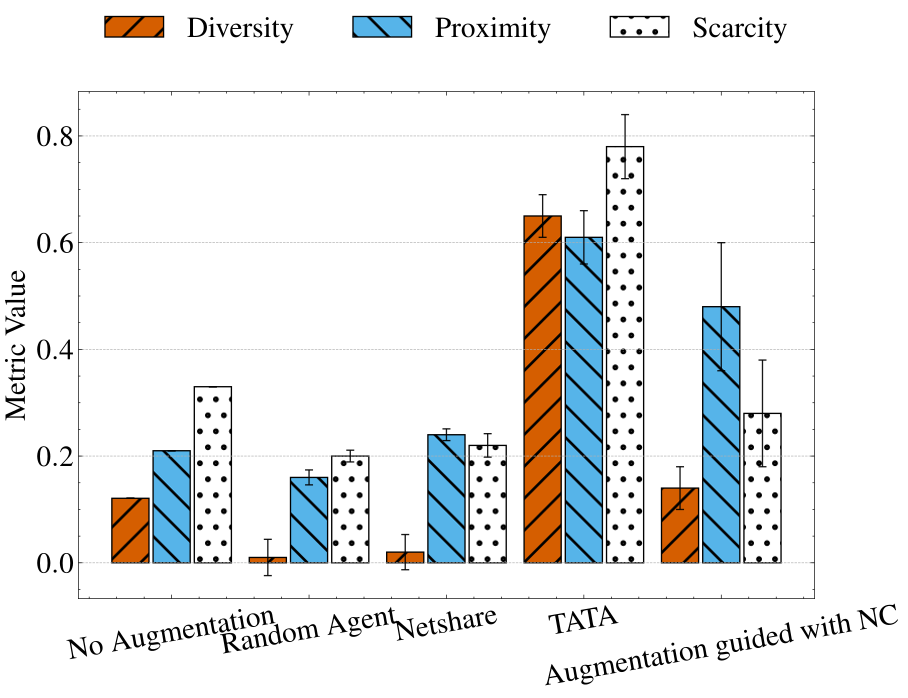
\includegraphics[width=\linewidth]{sections/TATA/results/figures/metrics_bars_grayscale_std-transparent.png}
			\caption{\scriptsize Test-set quality metrics (higher is more challenging/covered).}
			\label{fig:aug}
		\end{figure}
	\end{columns}
\end{frame}


\begin{frame}{Test-set Augmentation — Impact on NIDS}
	\small
	\begin{columns}[T,onlytextwidth]
		% ---------------- Left column ----------------
		\column{0.55\linewidth}
		\begin{itemize}
			\item \textbf{NIDS impact (RF example):}
			      \begin{itemize}

				      \item \textbf{TATA:} Precision \textcolor{red!70!black}{--\(\sim\)46\%}; Recall
				            \textcolor{red!70!black}{--\(\sim\)13\%}
				      \item[]
				      \item \textbf{NC:} Precision \textcolor{red!70!black}{--\(\sim\)23\%}; Recall
				            \textcolor{red!70!black}{--\(\sim\)16\%}
			      \end{itemize}
			\item[]
			\item \textbf{Note:} higher scarcity spreads errors across boundaries
			      \(\Rightarrow\) FP \(\uparrow\) \(\Rightarrow\) precision \(\downarrow\).
			\item[]
			\item \(\Rightarrow\) \textbf{proximity is the key driver;}
			      scarcity and diversity are complementary (spread errors, avoid redundancy)

		\end{itemize}

		% ---------------- Right column ----------------
		\column{0.42\linewidth}
		\centering
		\begin{figure}
			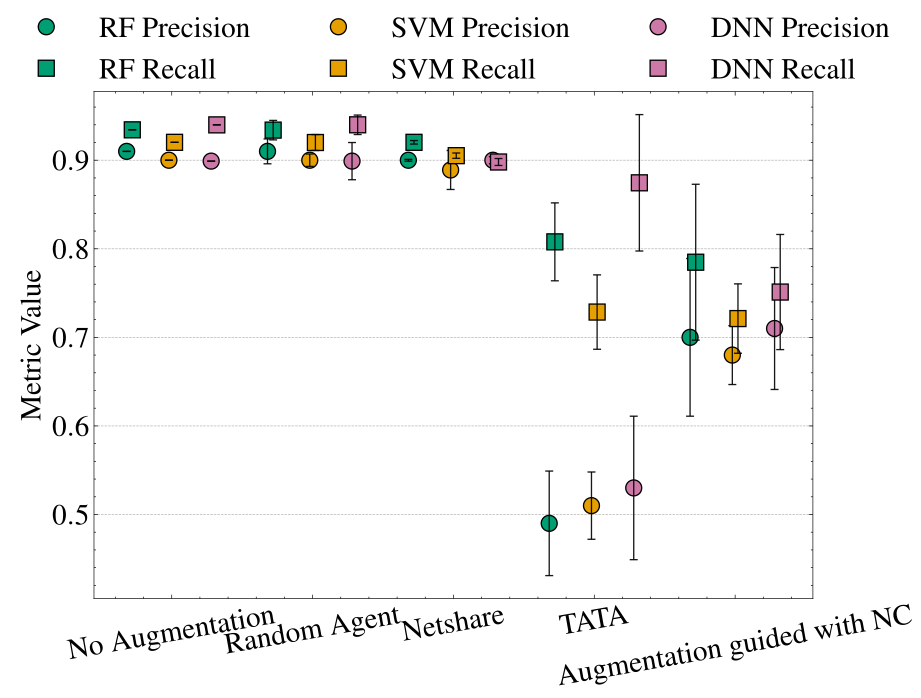
\includegraphics[width=\linewidth]{sections/TATA/results/figures/nids_performance_grayscale_std-transparent.png}
			\caption{\scriptsize Impact on detection metrics (example: RF).}\label{fig:figure}
		\end{figure}
	\end{columns}
\end{frame}


%\begin{frame}{Test-set Augmentation Evaluation}
%  \scriptsize
%  \begin{columns}[T,onlytextwidth]
%    % ---------------- Left column (adds content over time) ----------------
%    \column{0.55\linewidth}
%    \begin{itemize}
%      \item<1-> \textbf{Protocol:}
%      20 eval episodes on IDS2017; no reward/updates; add Benign SSH flows;
%      report mean$\pm$sd.
%
%      \item<1-> \textbf{Baselines:} Random, NetShare (GAN), RL\,+\,Neuron Coverage (NC).
%
%      \item<2-> \textbf{Quality metrics:}
%      \begin{itemize}
%        \scriptsize
%        \item<2-> \textbf{TATA:} \(D\) \textcolor{green!60!black}{\(+\sim 437\%\)}; \(P\)
%        \textcolor{green!60!black}{\(+\sim 190\%\)}; \(S\)
%        \textcolor{green!60!black}{\(+\sim 136\%\)}
%        \item<2-> \textbf{NC:} \(D\) \textcolor{gray!60!black}{\(\approx 0\)}; \(P\)
%        \textcolor{green!60!black}{\(+\sim 129\%\)}; \(S\)
%        \textcolor{gray!60!black}{\(\approx 0\)}
%        \item<2-> \textbf{Random/NetShare:} \(D\)
%        \textcolor{red!70!black}{\(\downarrow\) to \(\approx 0\)}; \(P\)
%        \textcolor{gray!60!black}{\(\approx 0\)}; \(S\)
%        \textcolor{red!70!black}{\(\downarrow\)}
%      \end{itemize}
%
%      \item<3-> \textbf{NIDS impact:}
%      \begin{itemize}
%        \scriptsize
%        \item<3-> \textbf{TATA (RF example):} Precision
%        \textcolor{red!70!black}{--\(\sim\)46\%}; Recall
%        \textcolor{red!70!black}{--\(\sim\)13\%}
%        \item<3-> \textbf{NC (RF example):} Precision
%        \textcolor{red!70!black}{--\(\sim\)23\%}; Recall
%        \textcolor{red!70!black}{--\(\sim\)16\%}
%        \item<3-> \textbf{Note:} higher scarcity spreads errors across boundaries
%        \(\Rightarrow\) FP \(\uparrow\) \(\Rightarrow\) precision \(\downarrow\).
%      \end{itemize}
%    \end{itemize}
%
%    % ---------------- Right column (figure swaps on step 3) ----------------
%    \column{0.42\linewidth}
%    \centering
%    \only<1-2>{%
%      \begin{figure}
%        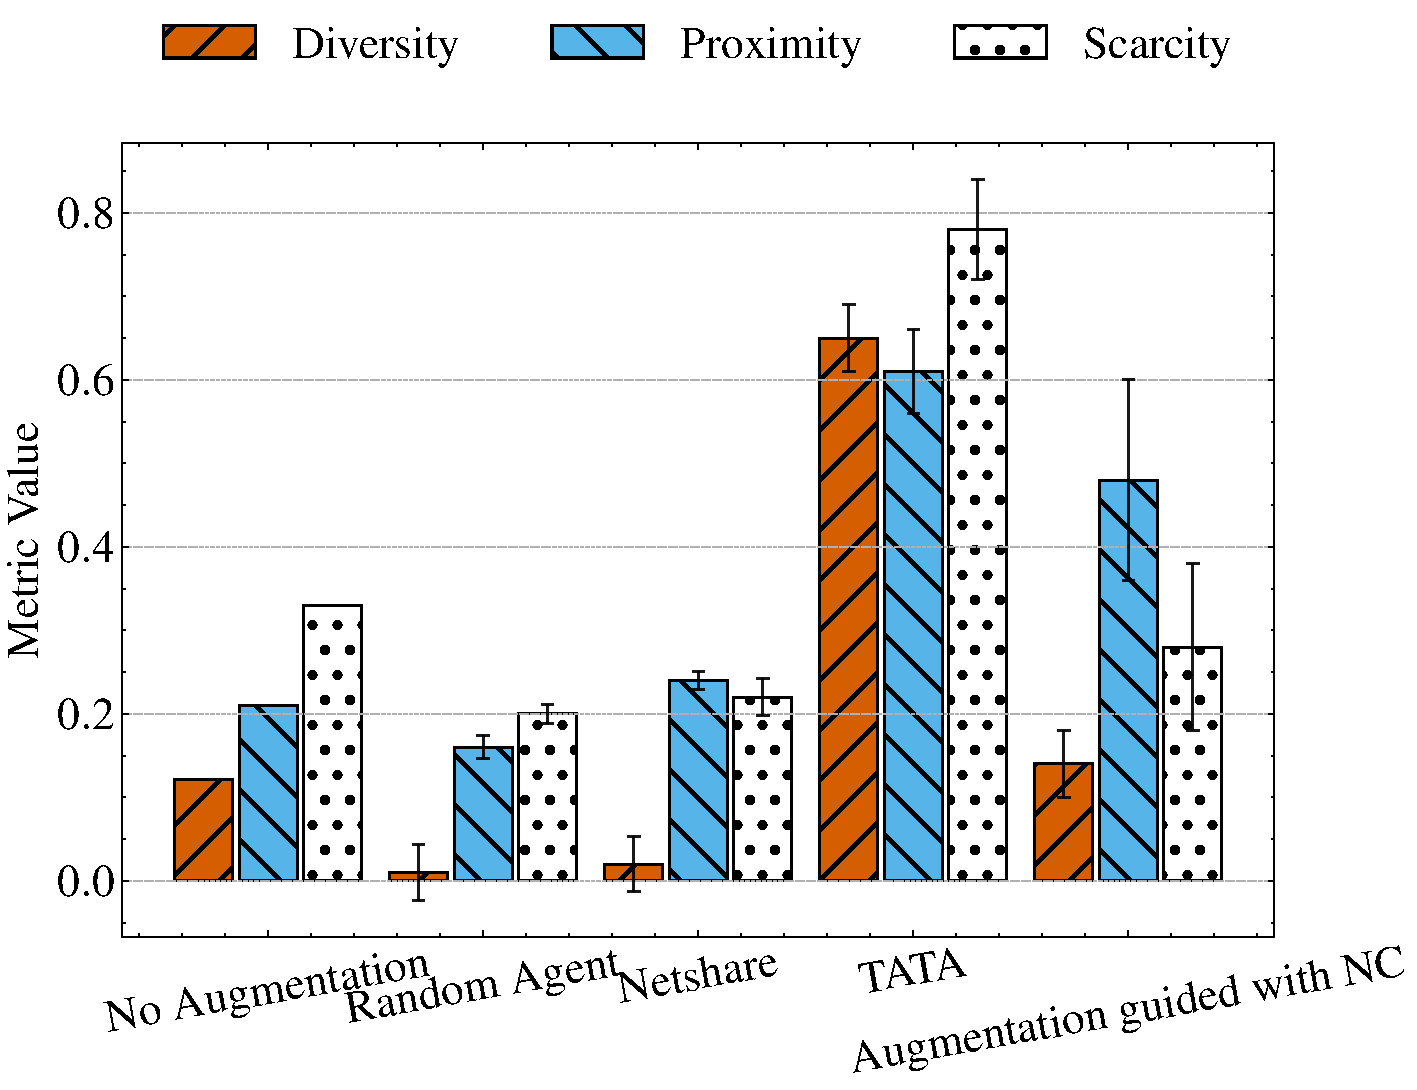
\includegraphics[width=\linewidth]{results/figures/metrics_bars_grayscale_std}
%        \label{fig:test_set_aug_metrics}
%      \end{figure}
%    }
%    \only<3->{%
%      \begin{figure}
%        \includegraphics[width=\linewidth]
%        {results/figures/nids_performance_grayscale_std}% <-- replace with your impact
%        \label{fig:test_set_aug_impact}
%      \end{figure}
%    }
%  \end{columns}
%\end{frame}
%\begin{frame}{Test-set Augmentation Evaluation}
%  \scriptsize
%  \begin{columns}[T,onlytextwidth]
%    % ---------------- Left column ----------------
%    \column{0.55\linewidth}
%
%    % (1) Protocol + Baselines
%    \only<1>{
%      \textbf{Protocol:} 20 eval episodes on IDS2017; no reward/updates; add Benign SSH
%      flows; report mean$\pm$sd.\\[0.4em]
%      \textbf{Baselines:} Random, NetShare (GAN), RL\,+\,Neuron Coverage (NC).
%    }
%
%    % (2) Quality metrics
%    \only<2>{
%      \textbf{Quality metrics:}
%      \begin{itemize}
%        \scriptsize
%        \item \textbf{TATA:} \(D\) \textcolor{green!60!black}{\(+\sim 437\%\)};\; \(P\)
%        \textcolor{green!60!black}{\(+\sim 190\%\)};\; \(S\)
%        \textcolor{green!60!black}{\(+\sim 136\%\)}
%        \item \textbf{NC:} \(D\) \textcolor{gray!60!black}{\(\approx 0\)};\; \(P\)
%        \textcolor{green!60!black}{\(+\sim 129\%\)};\; \(S\)
%        \textcolor{gray!60!black}{\(\approx 0\)}
%        \item \textbf{Random/NetShare:} \(D\)
%        \textcolor{red!70!black}{\(\downarrow\) to \(\approx 0\)};\; \(P\)
%        \textcolor{gray!60!black}{\(\approx 0\)};\; \(S\)
%        \textcolor{red!70!black}{\(\downarrow\)}
%      \end{itemize}
%    }
%
%    % (3) NIDS impact
%    \only<3>{
%      \textbf{NIDS impact:}
%      \begin{itemize}
%        \scriptsize
%        \item \textbf{TATA (RF example):} Precision
%        \textcolor{red!70!black}{--\(\sim\)46\%};\; Recall
%        \textcolor{red!70!black}{--\(\sim\)13\%}
%        \item \textbf{NC (RF example):} Precision \textcolor{red!70!black}{--\(\sim\)
%23\%}
%        ;\; Recall \textcolor{red!70!black}{--\(\sim\)16\%}
%        \item \textbf{Note:} higher scarcity spreads errors across boundaries
%        \(\Rightarrow\) FP \(\uparrow\) \(\Rightarrow\) precision \(\downarrow\).
%      \end{itemize}
%    }
%
%    % ---------------- Right column ----------------
%    \column{0.42\linewidth}
%    \centering
%    \only<1-2>{%
%      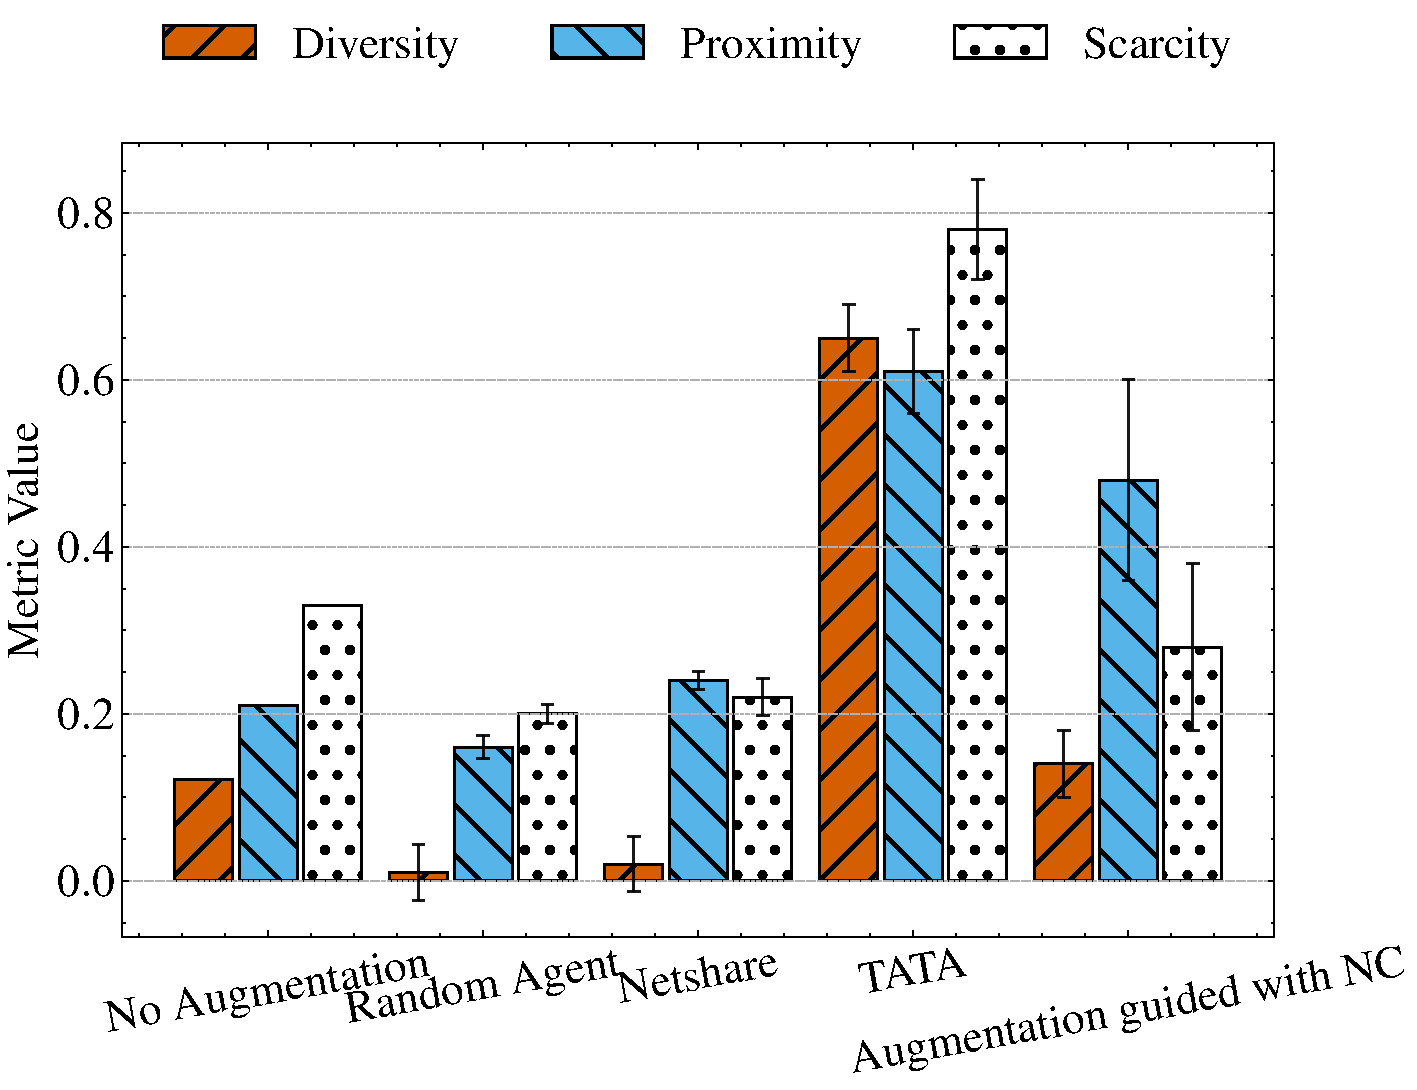
\includegraphics[width=\linewidth]{results/figures/metrics_bars_grayscale_std}%
%    }
%    \only<3->{%
%      \includegraphics[width=\linewidth]
%      {results/figures/nids_performance_grayscale_std}
%    }
%  \end{columns}
%\end{frame}


%\begin{frame}
%{Test set Augmentation Evaluation}
%
%
%  \small
%  \begin{columns}[T,onlytextwidth]
%    \column{0.55\linewidth}
%    \begin{itemize}
%      \item \textbf{Reward ablation:} train with single metrics or pairs: \(D\),
%      \(P\), \(S\), \(D{+}P\), \(P{+}S\), \(S{+}D\).
%      \item \textbf{Result:} any combo including \(P\) (\(P\), \(P{+}S\),
%      \(D{+}P\)) stresses NIDS most; others have minor impact.
%      \item \textbf{Example (RF):} \(P{+}S\) → recall \(0.934\!\to\!0.862\) (
%      \(-\sim8\%\)), precision \(0.910\!\to\!0.460\) (\(-\sim49\%\)); \(S{+}D\)
%      → recall \(-\sim4\%\), precision \(-\sim3\%\).
%      \item \textbf{Takeaway:} \(P\) is the key driver; \(S,D\)
%      are complementary (spread errors, avoid redundancy).
%    \end{itemize}
%
%    \column{0.42\linewidth}
%    \centering
%    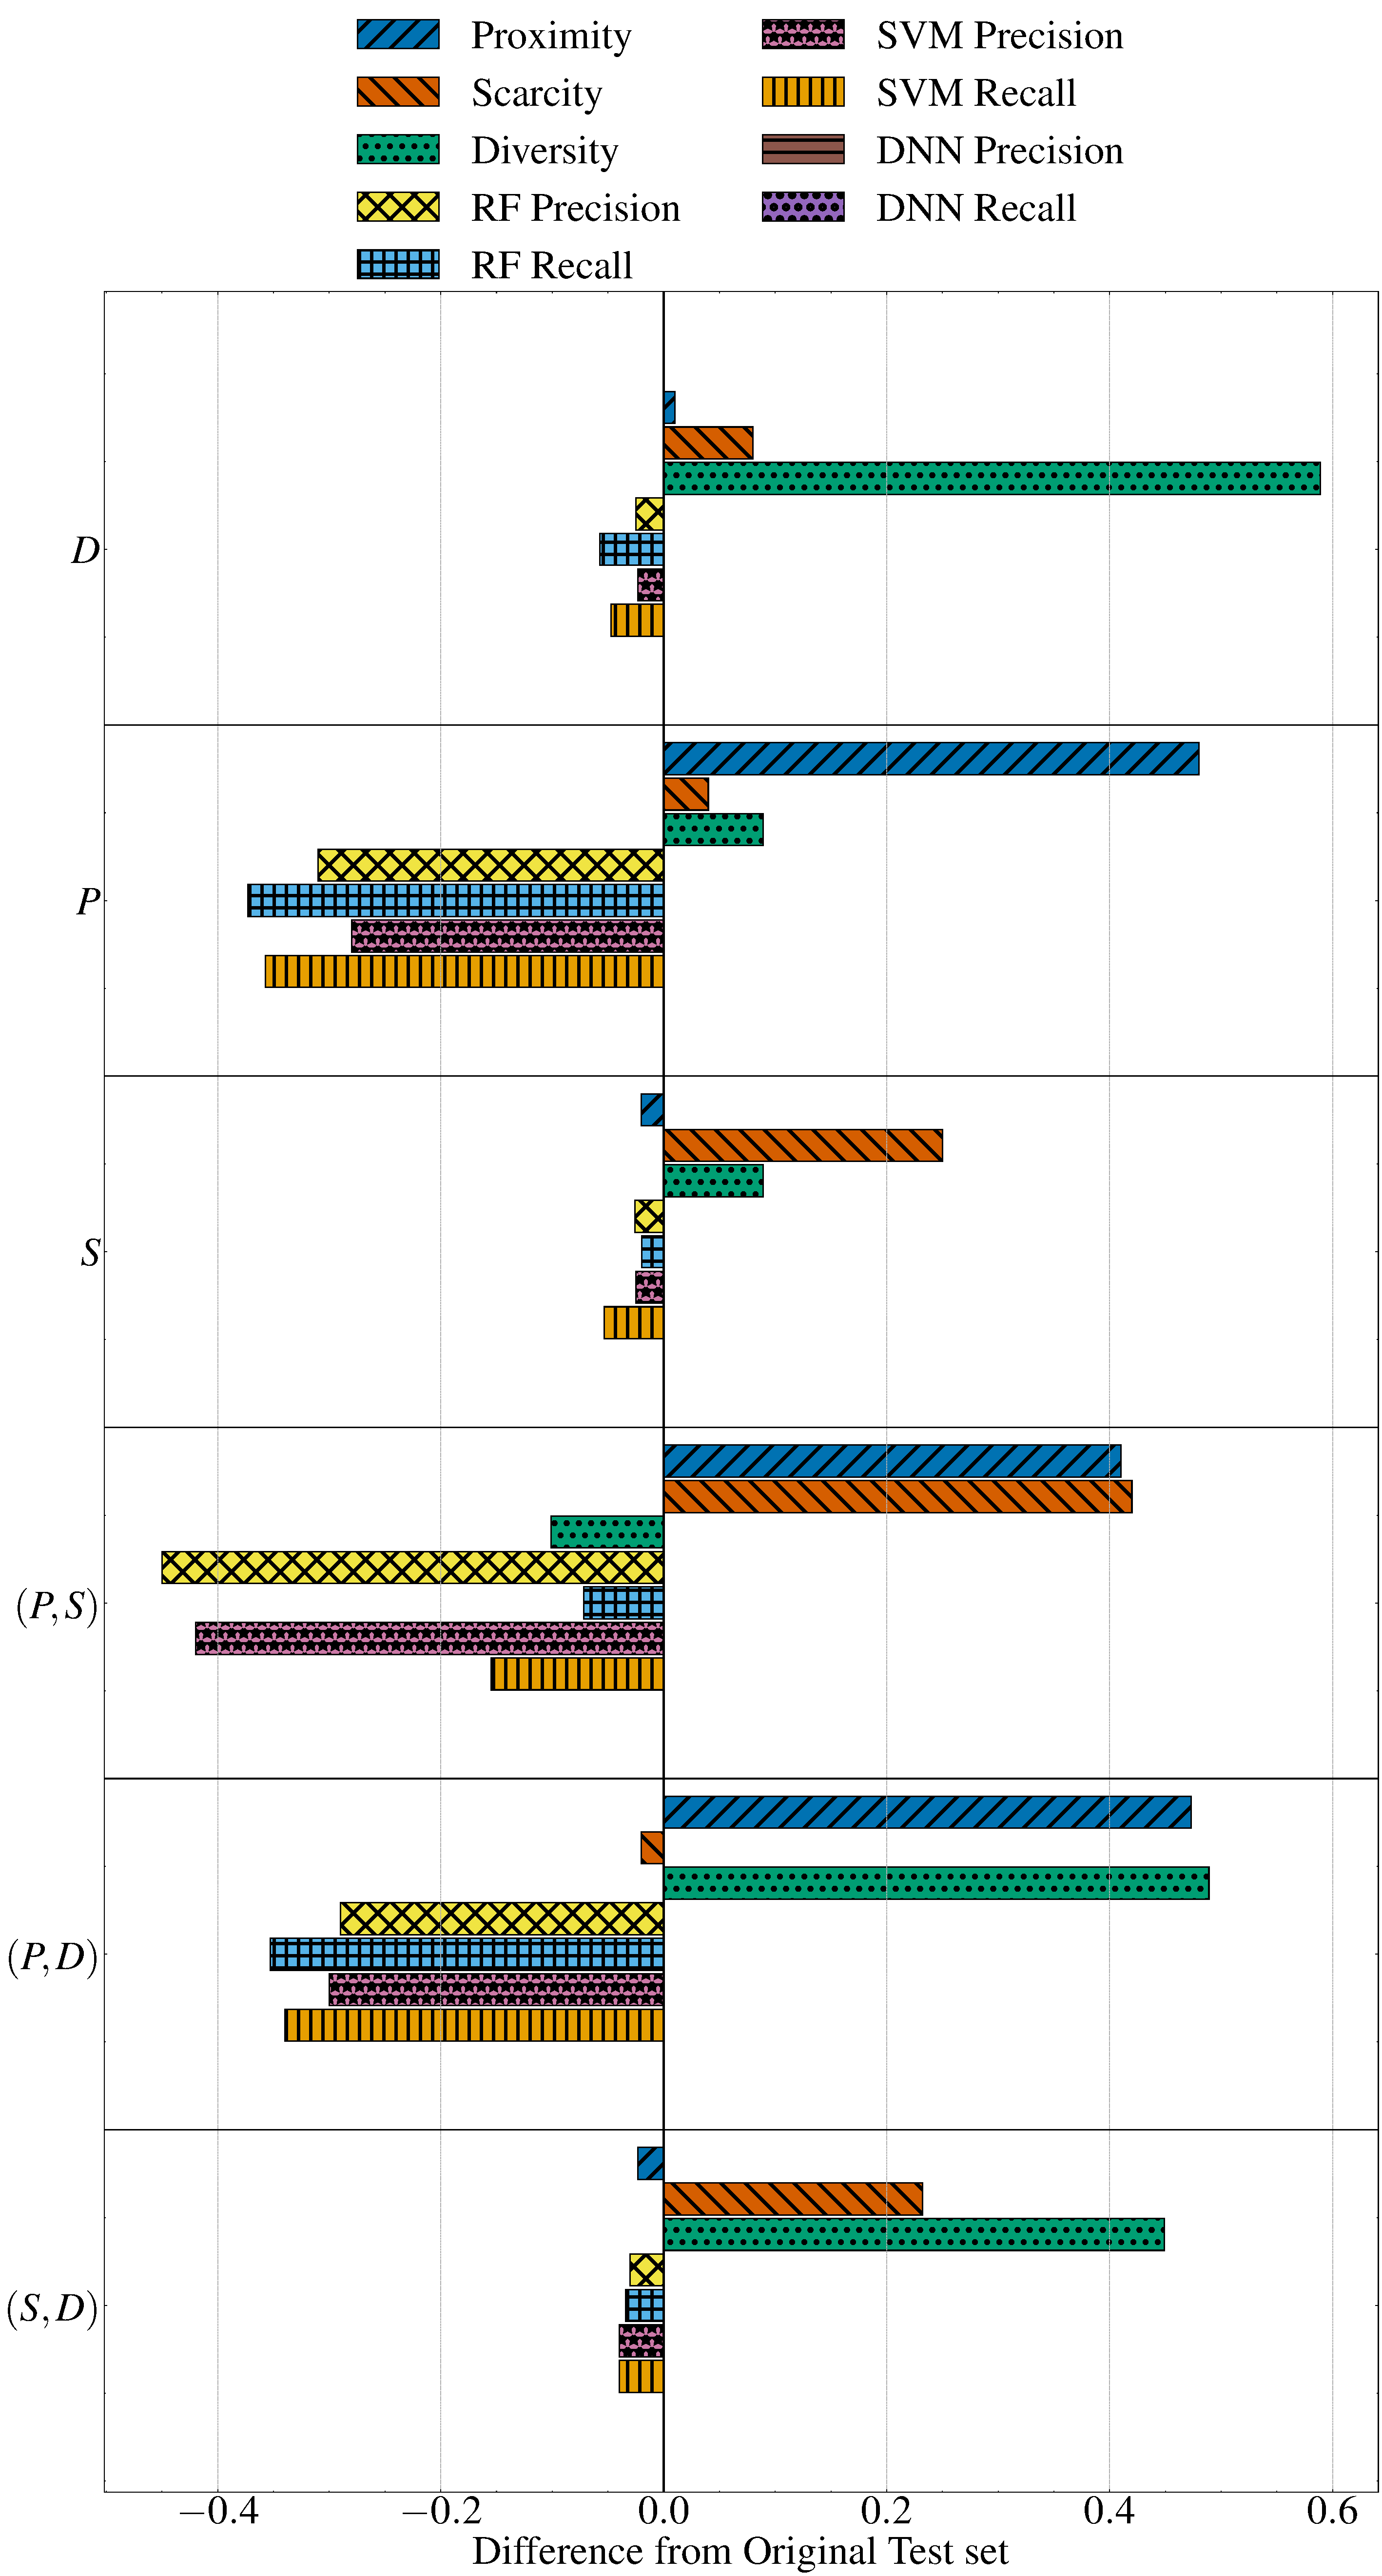
\includegraphics[width=0.7\linewidth]{results/figures/centered_bars_diff}
%  \end{columns}
%
%\end{frame}

\begin{frame}{Datasets Analysis}

	\small
	\begin{columns}[T,onlytextwidth]
		\column{0.55\linewidth}
		\begin{itemize}
			\item Apply \(D,P,S\)
			      across many NIDS datasets (2009–2020), sorted by release year; averages
			      over ten 60/20 splits.
			\item []
			\item No increasing pattern; values mostly \(\le 0.5\)
			      with occasional peaks (e.g., early IDS2017/2018); low within-dataset variation.
			\item []
			\item \(\Rightarrow\)
			      Despite richer, newer testbeds, NIDS test-set difficulty hasn’t
			      substantially increased. (CV refs like MNIST/CIFAR-10 score higher on
			      \(D,P,S\).)
		\end{itemize}
		\column{0.42\linewidth}
		\begin{figure}
			\centering
			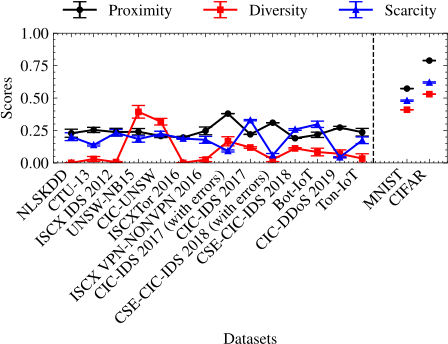
\includegraphics[width=\linewidth]{sections/TATA/results/figures/datasets_analysis-crop-transparent.png}
			\caption{\scriptsize Test-set assessment of NIDS datasets.}
			\label{fig:datasets_analysis}
		\end{figure}
	\end{columns}

\end{frame}


\begin{frame}{Part II conclusion}
	\small
	\begin{columns}[T,onlytextwidth]
		\column{0.57\linewidth}
		\begin{itemize}
			\setlength\itemsep{1em}
			\item[]
			      \tataGapClosureVisual
			\item Across public NIDS benchmarks, metrics remain mostly below \textbf{0.5} \(\Rightarrow\) limited test-set difficulty.
		\end{itemize}

		\column{0.40\linewidth}
		\centering
		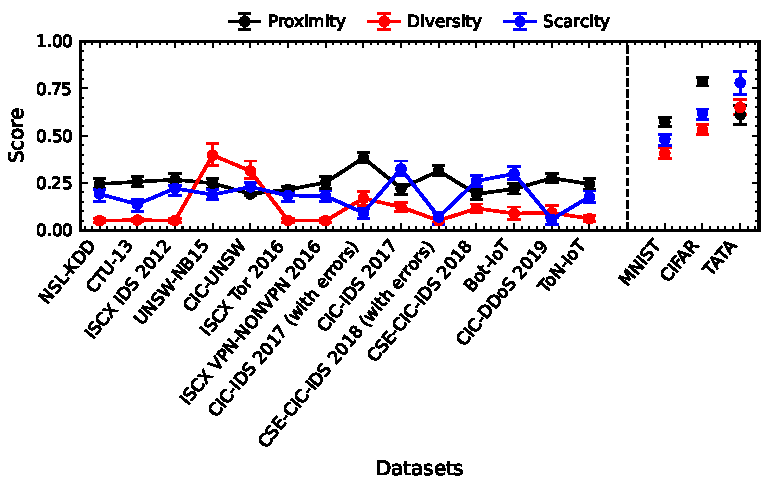
\includegraphics[width=\linewidth]{sections/TATA/results/figures/datasets_analysis_scienceplots.pdf}
		\par\vspace{0.25em}
		{\scriptsize Public NIDS benchmarks ordered on the x-axis by release year (2009--2020)}
	\end{columns}
\end{frame}
